\subsection{Localisation Changes of Human IFITs} \label{Localisation Changes of Human IFITs}
Asdfasfsdfasdf \newline
IF Mock | INF | Infection \newline
A549 BEAS2B

Merge pictures of clusters of cells looking at changes between subcellular localisation and a clear increase in mean intensity. Graphs show mean intensity changes from all cells imaged.

\begin{figure}
    \centering
    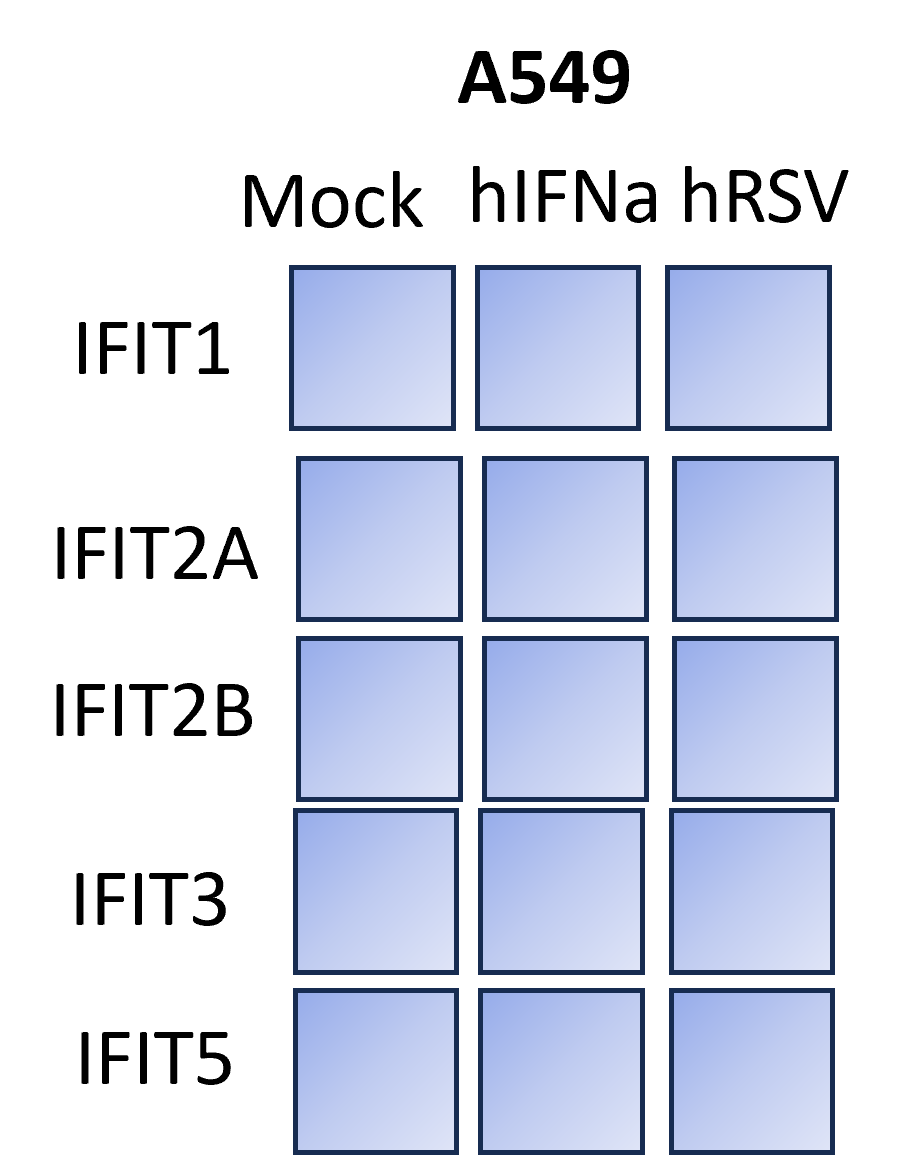
\includegraphics[width=1\linewidth]{06. Chapter 1/Figs/02. Localisation/01. a549 merges.png}
    \caption[A549 localisation mergers.]{A549 localisation mergers.}
    \label{A549 localisation mergers.}
\end{figure}


\begin{figure}
    \centering
    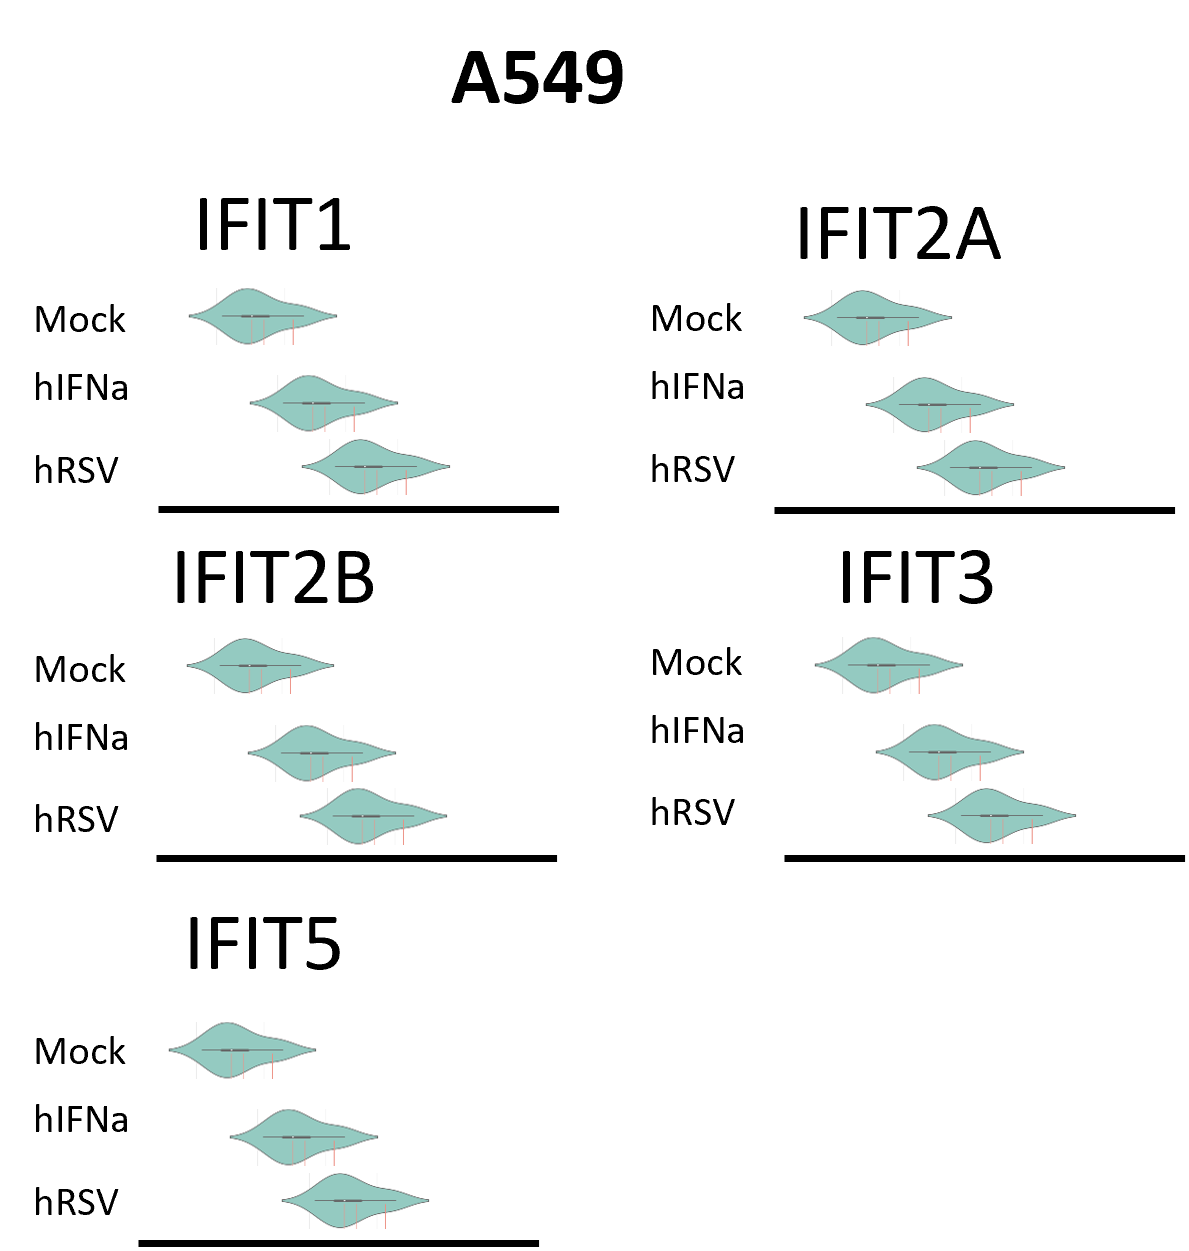
\includegraphics[width=1\linewidth]{06. Chapter 1/Figs/02. Localisation/02. a549 plots.png}
    \caption[A549 localisation plots.]{A549 localisation plots.}
    \label{A549 localisation plots.}
\end{figure}


\begin{figure}
    \centering
    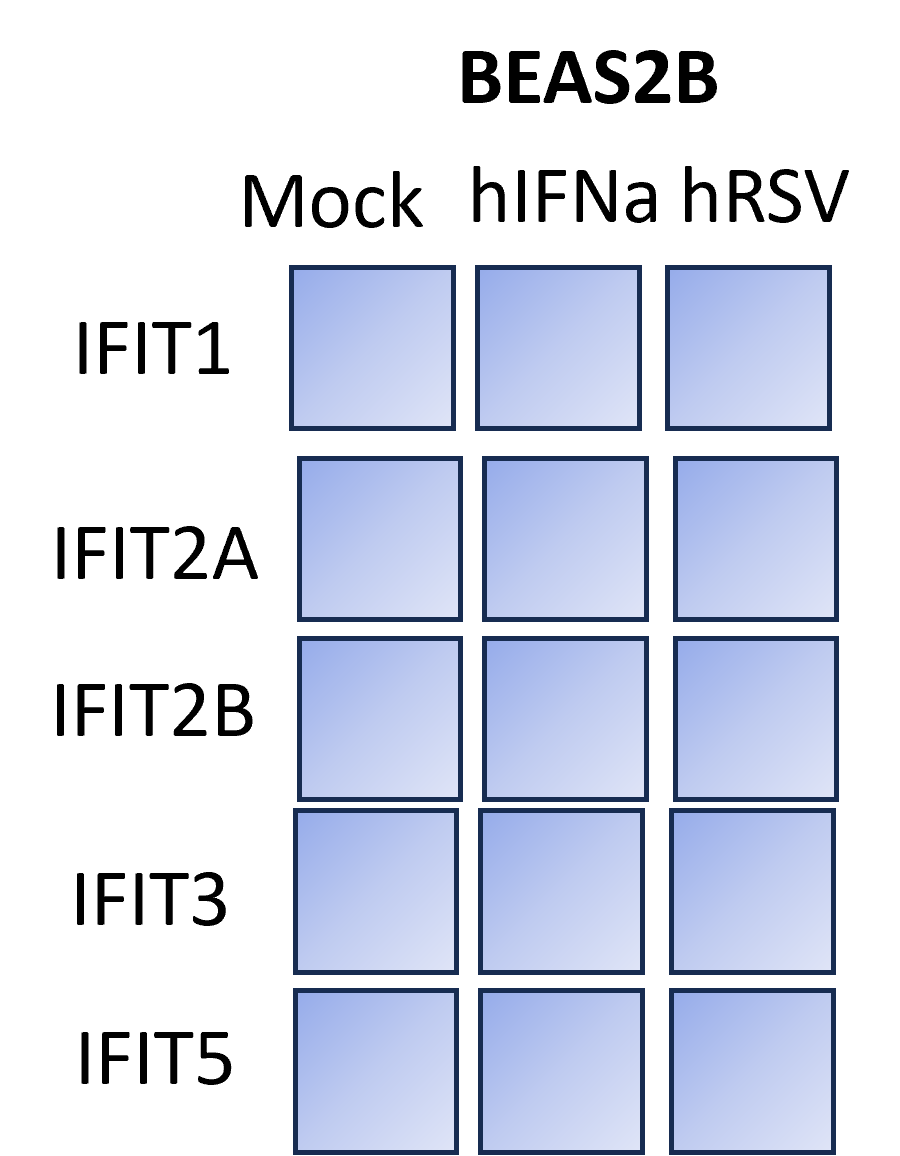
\includegraphics[width=1\linewidth]{06. Chapter 1/Figs/02. Localisation/03. beas2b merges.png}
    \caption[BEAS-2B localisation mergers.]{BEAS-2B localisation mergers.}
    \label{BEAS-2B localisation mergers.}
\end{figure}


\begin{figure}
    \centering
    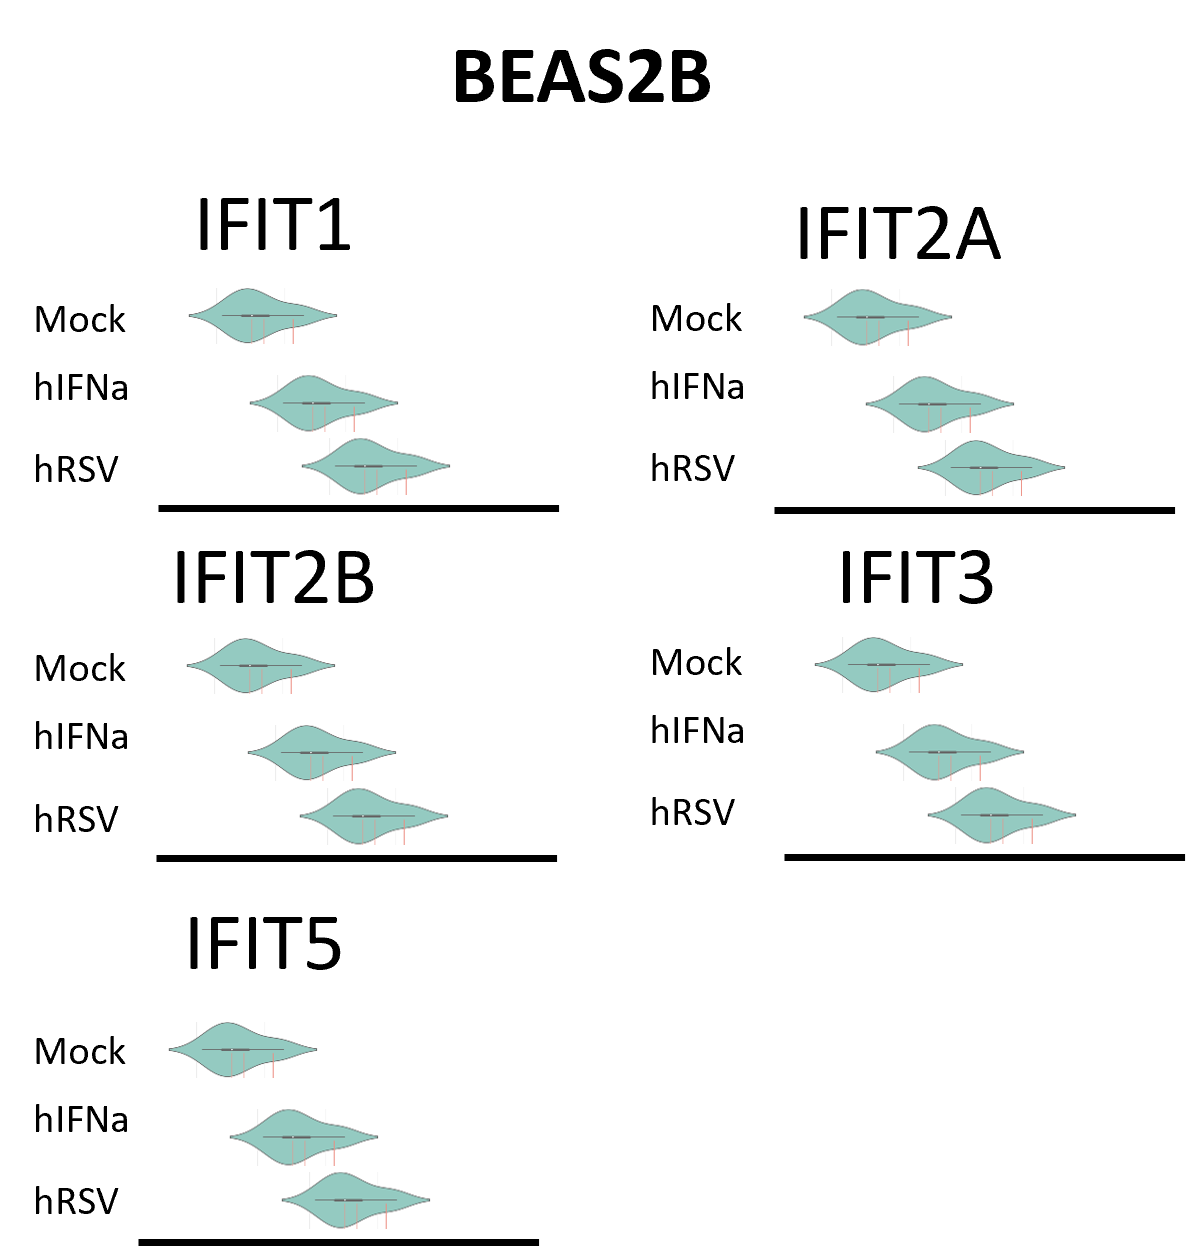
\includegraphics[width=1\linewidth]{06. Chapter 1/Figs/02. Localisation/04. beas2b plots.png}
    \caption[BEAS-2B localisation plots.]{BEAS-2B localisation plots.}
    \label{BEAS-2B localisation plots.}
\end{figure}


\subsubsection*{Summary} \label{Summary-human-localisation}
i guess tie it all togeher
